\documentclass{article}

\usepackage{fancyhdr} % Required for custom headers
\usepackage{lastpage} % Required to determine the last page for the footer
\usepackage{extramarks} % Required for headers and footers
\usepackage[usenames,dvipsnames]{color} % Required for custom colors
\usepackage{graphicx} % Required to insert images
\usepackage{listings} % Required for insertion of code
\usepackage{courier} % Required for the courier font
\usepackage{lipsum} % Used for inserting dummy 'Lorem ipsum' text into the template
\usepackage{hyperref}
\usepackage{multirow}
\usepackage{tabularx}
\usepackage{framed}
\usepackage{longtable}
\usepackage{listings}
\usepackage{subfigure}
\usepackage{afterpage}
\usepackage{amsmath,amssymb}            
\usepackage{rotating}  
\usepackage{fancyhdr}
\usepackage{graphicx}
\usepackage{amsthm}
\usepackage[scriptsize]{caption} 
\hyphenation{a-gen-tiz-za-zio-ne}
% Margins
\topmargin=-0.45in
\evensidemargin=0in
\oddsidemargin=0in
\textwidth=6.5in
\textheight=9.0in
\headsep=0.25in

\linespread{1.1} % Line spacing

\lstset{
  numbers=left,
  stepnumber=5,    
  firstnumber=1,
  numberfirstline=true
}

% Set up the header and footer
\pagestyle{fancy}
\lhead{\hmwkAuthorName} % Top left header
\chead{\hmwkClass\ (\hmwkClassInstructor\ \hmwkClassTime): \hmwkTitle} % Top center head
\rhead{\firstxmark} % Top right header
\lfoot{\lastxmark} % Bottom left footer
\cfoot{} % Bottom center footer
\rfoot{Page\ \thepage\ of\ \protect\pageref{LastPage}} % Bottom right footer
\renewcommand\headrulewidth{0.4pt} % Size of the header rule
\renewcommand\footrulewidth{0.4pt} % Size of the footer rule

\setlength\parindent{0pt} % Removes all indentation from paragraphs

\usepackage{listings}
\usepackage{color}

\definecolor{dkgreen}{rgb}{0,0.6,0}
\definecolor{gray}{rgb}{0.5,0.5,0.5}
\definecolor{mauve}{rgb}{0.58,0,0.82}

\lstset{frame=tb,
  language=Java,
  aboveskip=3mm,
  belowskip=3mm,
  showstringspaces=false,
  columns=flexible,
  basicstyle={\small\ttfamily},
  numbers=none,
  numberstyle=\tiny\color{gray},
  keywordstyle=\color{blue},
  commentstyle=\color{dkgreen},
  stringstyle=\color{mauve},
  breaklines=true,
  breakatwhitespace=true
  tabsize=3
}

%----------------------------------------------------------------------------------------
%	DOCUMENT STRUCTURE COMMANDS
%	Skip this unless you know what you're doing
%----------------------------------------------------------------------------------------

% Header and footer for when a page split occurs within a problem environment
\newcommand{\enterProblemHeader}[1]{
\nobreak\extramarks{#1}{#1 continued on next page\ldots}\nobreak
\nobreak\extramarks{#1 (continued)}{#1 continued on next page\ldots}\nobreak
}

% Header and footer for when a page split occurs between problem environments
\newcommand{\exitProblemHeader}[1]{
\nobreak\extramarks{#1 (continued)}{#1 continued on next page\ldots}\nobreak
\nobreak\extramarks{#1}{}\nobreak
}




%----------------------------------------------------------------------------------------
%	NAME AND CLASS SECTION
%----------------------------------------------------------------------------------------

\newcommand{\hmwkTitle}{UML: Unified Modeling Language} % Assignment title
\newcommand{\hmwkDueDate}{Marted\`i,\ Aprile 5,\ 2016} % Due date
\newcommand{\hmwkClass}{Ingegneria del Software 1} % Course/class
\newcommand{\hmwkClassTime}{} % Class/lecture time
\newcommand{\hmwkClassInstructor}{Claudio Menghi, Alessandro Rizzi} % Teacher/lecturer
\newcommand{\hmwkAuthorName}{} % Your name

\newcounter{EsercizioCounter}
 \setcounter{EsercizioCounter}{1}


\newcommand{\Esercizio}[1]{
%\setlength{\fboxsep}{2pt}
\fbox{
   
  \parbox[t][]{\textwidth}{
   \vspace{2ex}
   \textbf{Esercizio \arabic{EsercizioCounter}}: #1
    \vspace{2ex}
    \refstepcounter{EsercizioCounter}
  }
}
}






%----------------------------------------------------------------------------------------

\begin{document}

\maketitle

%----------------------------------------------------------------------------------------
%	TABLE OF CONTENTS
%----------------------------------------------------------------------------------------

%\setcounter{tocdepth}{1} % Uncomment this line if you don't want subsections listed in the ToC

\newpage
\tableofcontents
\newpage

\section{Design Principles}
Mentre si progetta il software \`e necessario considerare i seguenti principi:
\begin{itemize}
\item \emph{Open Close Principle: le entit\`a software (classi, moduli e funzioni) devono essere aperti all'estensione e chiusi alle modifiche.}
Un design intelligente consente di aggiungere una funzionalita (aperti all'estensione) senza modificare il codice gi\`a sviluppato o con delle modifiche minimali (chiusi alle modifiche).
\item \emph{Dependency Invertion Principle: i moduli di alto livello non devono dipendere da quelli di basso livello ma da loro astrazioni.}
Quando si utilizzano moduli di basso livello (e.g., classi che consentono letture da file) i moduli di alto livello non devono dipendere direttamente da questi elementi; \`e consigliato aggiungere un livello di astrazione (High Level Classes $\rightarrow$ Abstraction Layer $\rightarrow$ Low Level Classes) in modo tale da consentire di cambiare agevolmente le Low Level Classes
\item \emph{Interface Segregation Principle: i moduli non devono dipendere da interfacce che non utilizzano} Non aggiungete nelle interfacce metodi che non servono.
\item \emph{Single Responsibility Principle: ogni classe deve avere solo una ragione per essere modificata} 
Questo principio specifica che ogni classe si deve occupare solamente di una funzionalit\`a. 
Se una classe si occupa di due funzionalit\`a significa che \`e necessario dividere la classe in due.
\item \emph{Liskov's Substitution Principle: le classi derivate mediante estensioni (una classe che ne estende un altra) deve essere completamente sostituibile alla classe di partenza}.
 
\end{itemize}

\section{Introduzione}
UML contiene un insieme di notazioni grafiche che supportano lo sviluppatore nelle diverse fasi di sviluppo del software. \`E composto da una serie di notazioni che consentono di specificare la maggior parte dei costrutti  forniti da un linguaggio orientato agli oggetti. Lo scopo di UML e' di fornire uno strumento  per descrivere (progettare) il sistema in fase di sviluppo e viene utilizzato al fine di:
\begin{itemize}
\item aiutare gli \emph{analisti} a capire le funzionalit\`a del sistema
\item \emph{progettare} il sistema
\item comunicare con i committenti
\end{itemize}
Di solito per scopi diversi vengono utilizzati modelli differenti.

Alcuni dei diagrammi piu' utilizzati sono:
\begin{itemize}
\item diagrammi di struttura: descrivono la ``\emph{struttura}" dell'applicazione in fase di sviluppo
\item diagrammi di comportamento: descrivono il ``\emph{comportamento}" dell'applicazione in fase di sviluppo
\end{itemize}

Questa esercitazione \`e focalizzata sui \emph{class diagrams} un particolare tipo di diagramma strutturale che consente di specificare l'architettura della soluzione proposta.

\subsection{Diagrammi delle classi}
Sono utilizzati per fornire una visione statica del sistema. Sono composti da classi e relazioni tra classi.
\begin{itemize}
\item \emph{classi}: definisce un insieme di oggetti (istanze) che hanno le stesse caratteristiche. Per esempio la classe macchina definisce la struttura che devono avere gli oggetti (istanze) di tipo macchina. Un oggetto \`e una specifica istanza di una classe, e.g., una specifica macchina.
\item \emph{relazioni}: definiscono delle dipendenze tra le diverse classi del sistema, in particolare esistono relazioni di uso, generalizzazione (ereditariet\`a) e associazione (due tipi specifici di associazione sono aggregazione e composizione).
\end{itemize}

\subsubsection{Classi}
Le classi descrivono un insieme di oggetti. Al fine di descrivere gli oggetti di una classe e' necessario specificare:
\begin{itemize}
\item \emph{Stato}: descrive un oggetto in uno specifico istante temporale. Lo stato viene descritto per mezzo di attributi.
\item \emph{Comportamento}: indicano i metodi che un oggetto pu\`o invocare. I comportameti sono descritti per mezzo di metodi. L'esecuzione di un metodo spesso comporta la modifica dello stato di un oggetto.
\end{itemize}
Ogni classe \`e rappresentata per mezzo di un rettangolo diviso verticalmente in tre parti contenenti il nome, gli attributi e
 i metodi dalla classe, rispettivamente.  
 Per esempio, la classe rappresentata in Figura~\ref{Fig:Classe} ha come nome \texttt{Persona}, ha come attributi \texttt{nome}, \texttt{cognome} e \texttt{dataNascita} e come metodi \texttt{siSposa()} e \texttt{compieAnni()}. Gli attributi seguono la notazione: \texttt{<modificatore di visibilit\`a> nome attributo : <tipo attributo>[= valore di default]}. 
Dove il modificatore di visibilit\`a pu\`o essere public (\texttt{+}), private (\texttt{-}), protected ($\#$) and package ($\sim$).
 I metodi seguono la notazione: \texttt{<modificatore di visibilit\`a> nome metodo (<parametro 1: tipo parametro1>, ...): <tipo di ritorno>}.
I modificatori di visibilit\`a sono gli stessi usati per gli attributi. 
Quando un attributo o un metodo \`e sottolineato, l'attributo o il metodo \`e \emph{statico}.
 
 \begin{figure}[h!]
  \centering
    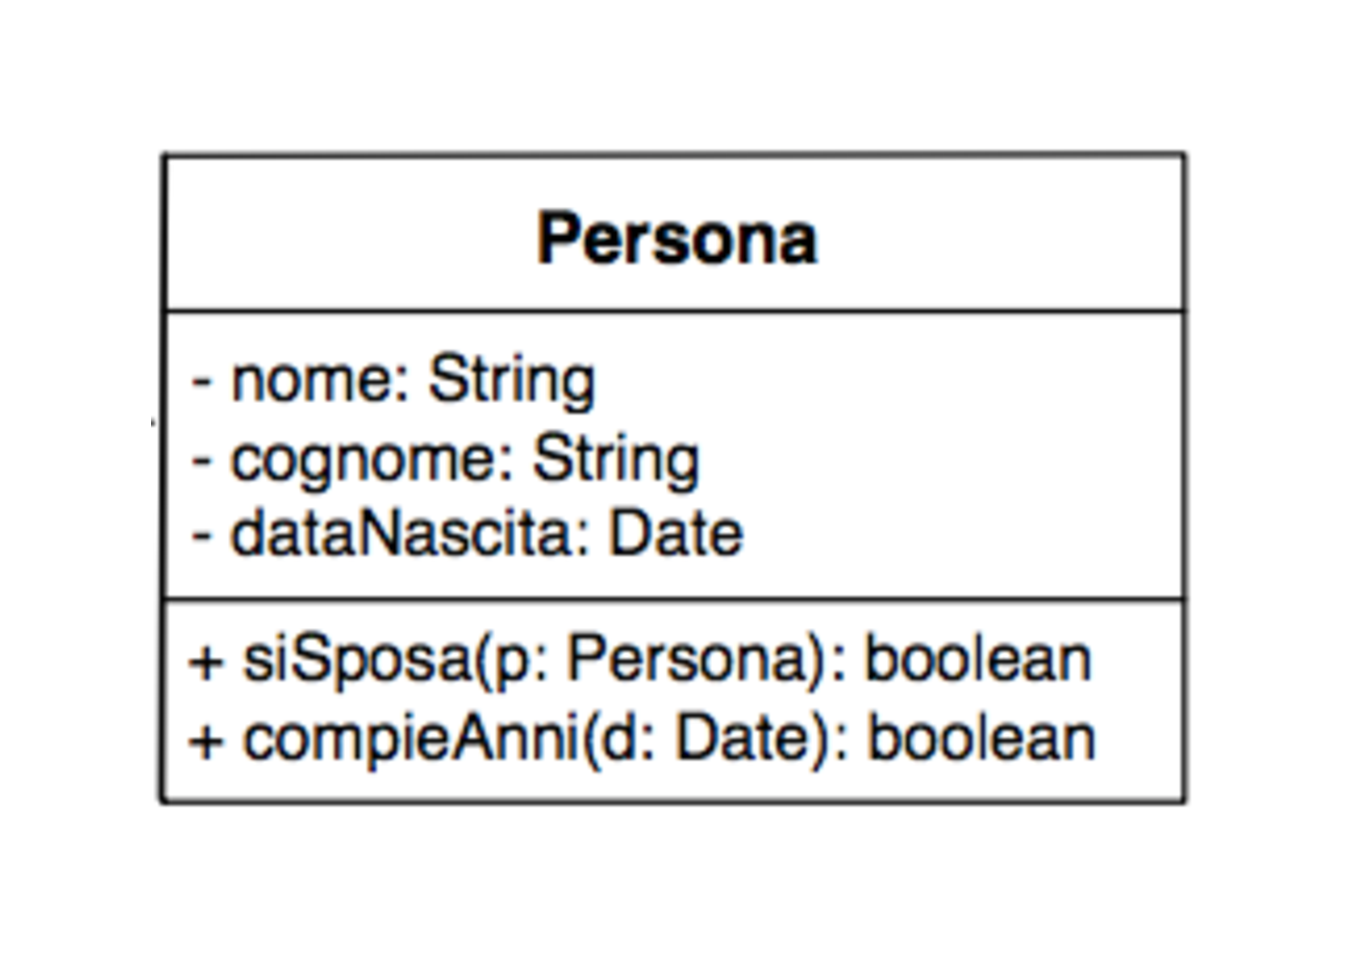
\includegraphics[width=0.3\textwidth]{Img/Persona.pdf}
      \caption{Una classe.}
      \label{Fig:Classe}
\end{figure}

 
La classe mostrata in Figura~\ref{Fig:Classe} \`e mappata nel codice Java presentato in seguito.
\begin{lstlisting}
public class Persona {
    private String nome;
    private String cognome;
    private Date dataNascita;
    
    public boolean siSposa(Persona p){
    }
    
    public boolean compieAnni(Date d){
    
    }
}
\end{lstlisting}

In un class diagram ci sono due modi possibili per indicare che una classe \`e astratta: scrivere il loro nome in \textit{italico} o indicarli per mezzo della dicitura   \{abstract\} indicata sotto il nome della classe.
\`E inoltre possibile specificare degli stereotipi sopra il nome della classe con la seguente sintassi: $\langle \langle stereotype \rangle \rangle$. Per esempio $\langle \langle interface \rangle \rangle$ indica che la classe specificata rappresenta un interfaccia mentre 
$\langle \langle utility \rangle \rangle$ indica che tutti i metodi o le variabili di una classe di tipo utility sono statiche.

\subsubsection{Associazione} 
\`E un tipo di relazione che descrive che due classi sono associate. Per esempio, Figura~\ref{Fig:Associazione} presenta un associazione tra le due classi \texttt{Persona} e \texttt{Casa}\footnote{Per semplicit\`a gli attributi e i metodi delle classi non sono mostrati nel diagramma}. 
L'associazione specifica la relazione \texttt{vive} la relazione tra le classi  \texttt{Persona} e \texttt{Casa}.  Solitamente il nome della relazione \`e un verbo. \`E anche possibile specificare alle estremit\`a i ruoli svolti dalle classi nell'associazione e anche una espressione che specifica la molteplicit\`a. La molteplicit\`a si riferice ai numeri posti sulle frecce e rappresentano il numero di oggetti connessi agli altri per mezzo dell'associazione. Le moltiplicit\`a possono essere espressi come numeri, ranges o combinazioni dei due.
\begin{itemize}
\item \textit{Digit}: il numero esatto di elementi
\item $*$ or $0..*$: zero o alcuni
\item $0..1$ Zero or one. In Java this is often implemented with a reference that can be null.
\item $1..*$ uno o molti
\item $3..5$ da 3 a 5 (in alcune varianti)
\end{itemize}
Per esempio in Figura~\ref{Fig:Associazione} viene specificato che una persona vive in una casa e che in una casa vive almeno una persona.
Gli estremi di un'associazione implicano la presenza di attributi impliciti. Per esempio il class diagram descritto in Figura~\ref{Fig:Associazione} viene mappato nel codice seguente.

\begin{figure}[h!]
  \centering
    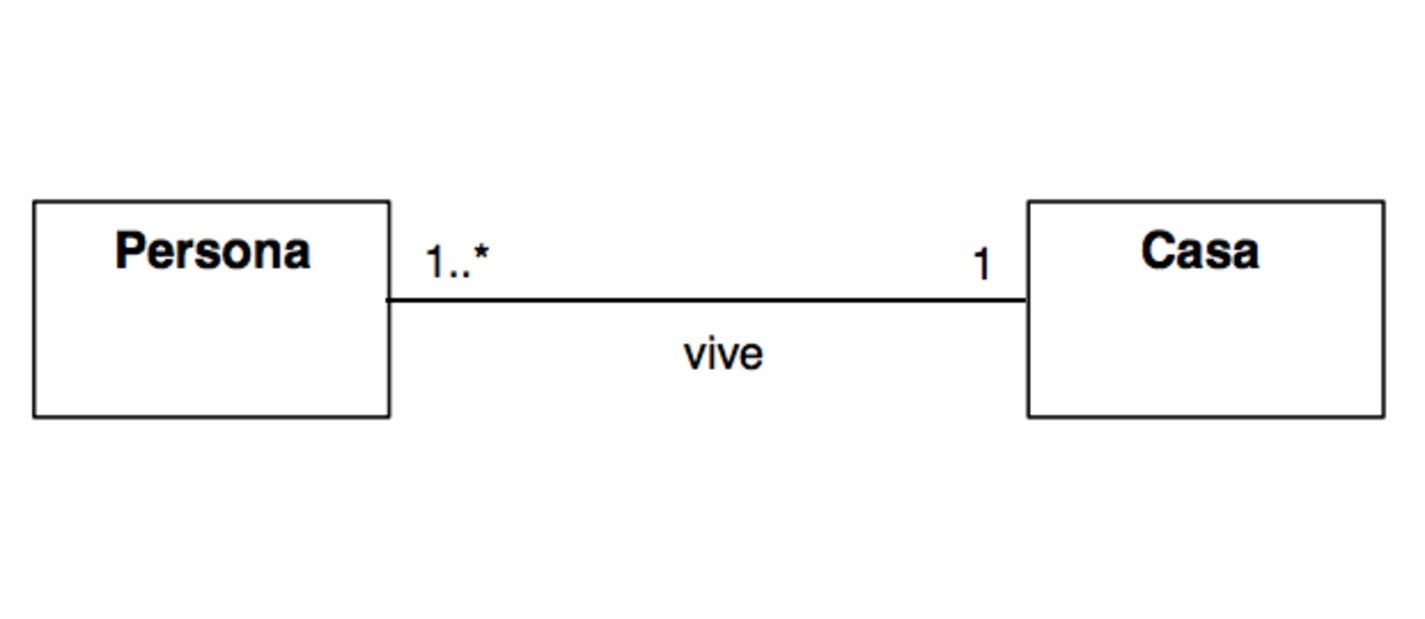
\includegraphics[width=0.5\textwidth]{Img/Associazione.pdf}
      \caption{Associazione tra Persona e Casa.}
      \label{Fig:Associazione}
\end{figure}

La classe \texttt{Persona} contiene il riferimento alla \texttt{Casa} della persona.

\begin{lstlisting}
public class Persona {
    private Casa casa; 
}
\end{lstlisting}
La classe \texttt{Casa} contiene una collezione di persone che vivono nella casa.
\begin{lstlisting}
public class Casa {
    private Collection<Persona> persone; 
}
\end{lstlisting}
\`E possibile specificare la direzione di navigabilit\`a dell'associazione. 
Per esempio, in Figura~\ref{Fig:Associazione2} l'associazione \`e navigabile solo nella direzione Casa$\rightarrow$Persona. Questo implica che data una casa \`e possibile sapere le persone che vivono in quella casa ma non viceversa. La nuova relazione viene mappata sul codice Java seguente:

\begin{figure}[h!]
  \centering
    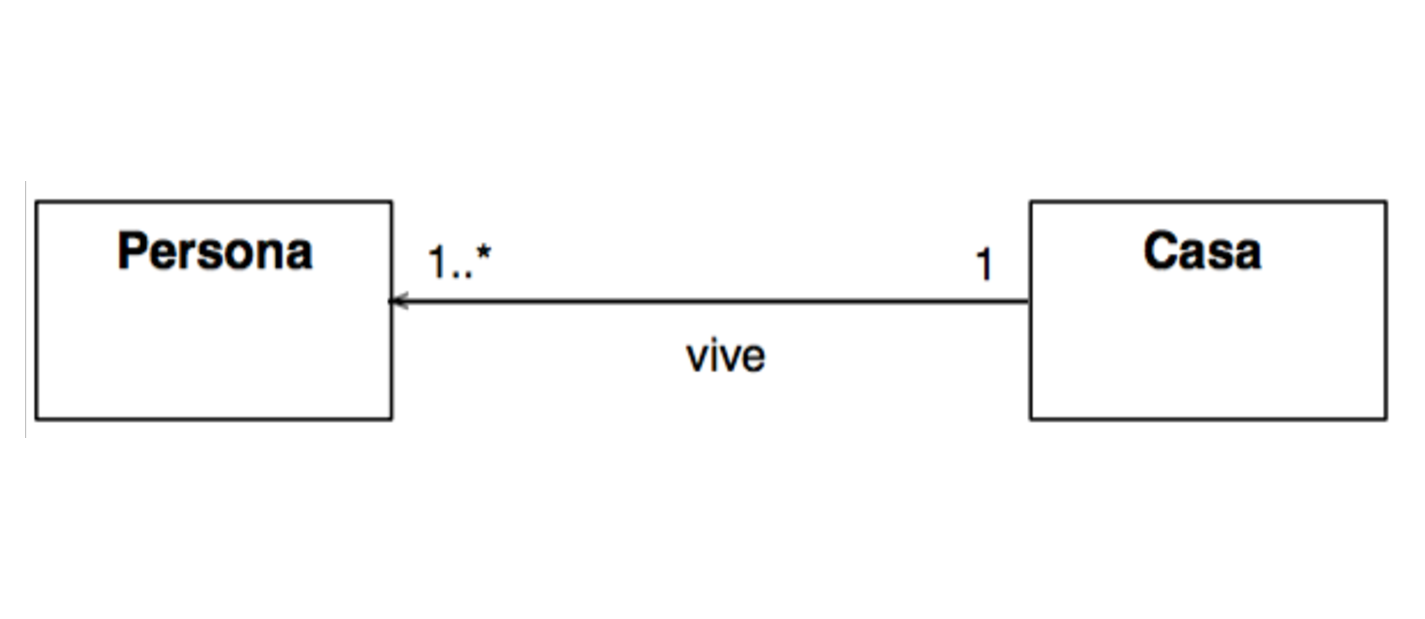
\includegraphics[width=0.5\textwidth]{Img/Associazione2.pdf}
      \caption{Associazione tra Persona e Casa.}
      \label{Fig:Associazione2}
\end{figure}

\begin{lstlisting}
public class Persona {
}
\end{lstlisting}
La classe \texttt{Casa} contiene una collezione di persone che vivono nella casa.
\begin{lstlisting}
public class Casa {
    private Collection<Persona> persone; 
}
\end{lstlisting}

L'aggregazione \`e un tipo specifico di associazione che descrive una relazione ``\`e una parte di". Nota che l'implementazione \`e indistinguibile da quella dell'associazione. Nell'esempio mostrato in Figura~\ref{Fig:Aggregazione}, un automobile aggrega un Telaio, un Motore e quattro Ruote. L'unica regola riguardante l'associazione consiste nel fatto che non \`e possibile creare cicli di aggregazioni. 

\begin{figure}[h!]
  \centering
    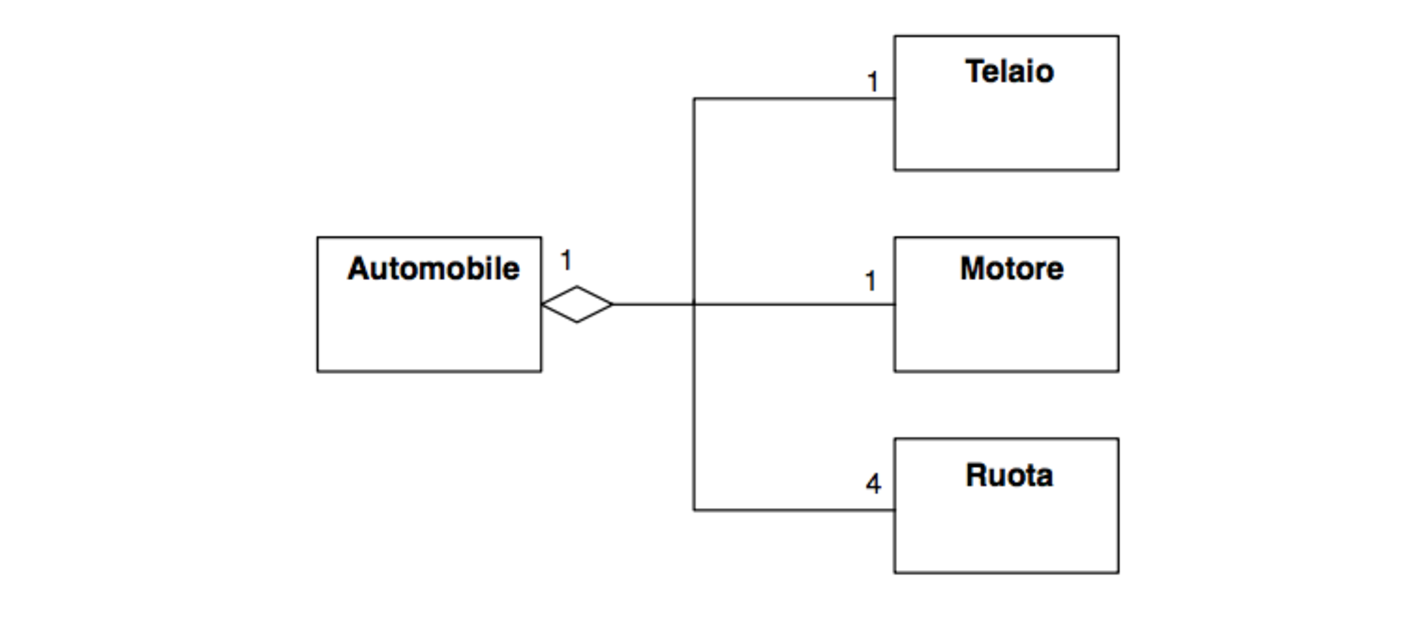
\includegraphics[width=0.7\textwidth]{Img/Aggregazione.pdf}
      \caption{Aggregazione tra Automobile, Telaio, Motore e Ruota.}
      \label{Fig:Aggregazione}
\end{figure}

\subsubsection{Composizione}
La composizione \`e un altro tipo speciale di associazione. La composizione indica che il contenitore \`e responsabile del ciclo vita del contenuto: se il contenitore \`e distrutto il contenuto deve essere distrutto con esso.
Nota che l'implementazione Java \`e indistinguibile da quella dell'associazione. Tuttavia, in questo caso, la ragione \`e un suo scarso utilizzo nella programmazione Java. \`E compito del programmatore garantire che quando il contenitore \`e distrutto il contenuto non deve essere pi\`u referenziato, ovvero deve essere rimosso dal garbage collector. Come per le aggregazioni non deve essere possibile creare cicli contenenti composizioni.
Nell'esempio mostrato in Figura~\ref{Fig:Composizione} quando la \texttt{Window} viene distrutta anche lo \texttt{Slider}, il \texttt{Panel} e il \texttt{Button} associati sono distrutti con essa.

\begin{figure}[h!]
  \centering
    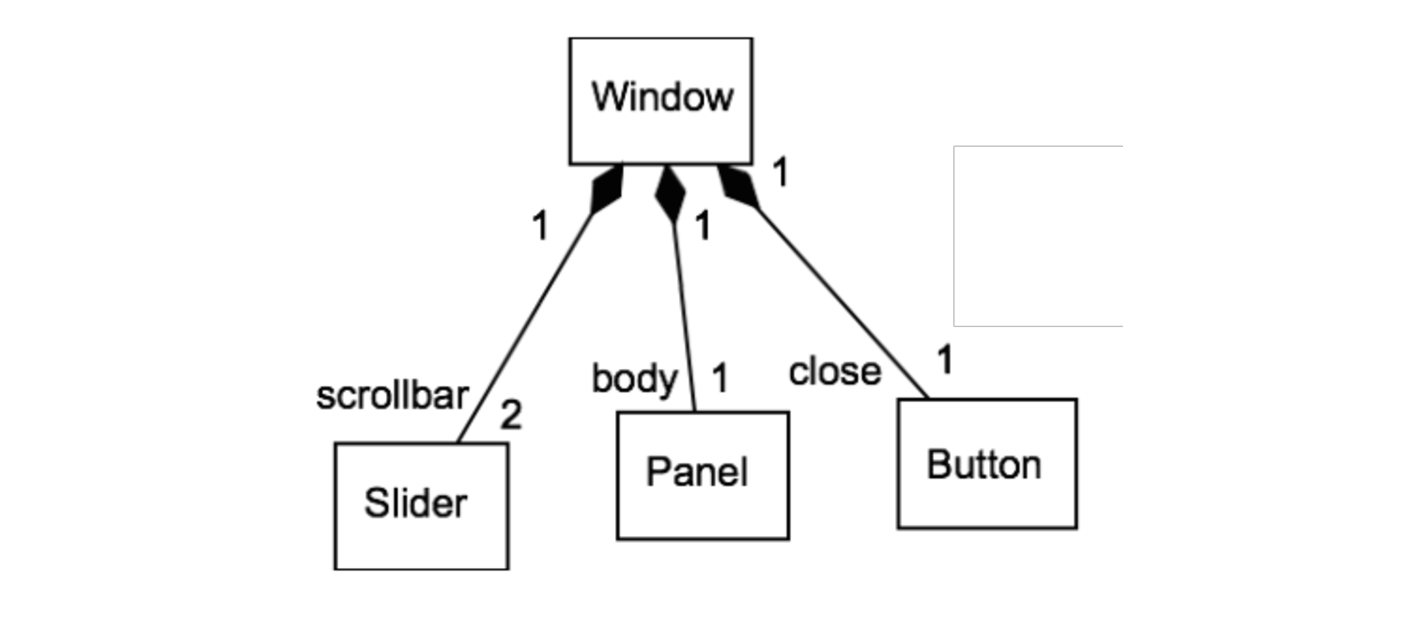
\includegraphics[width=0.7\textwidth]{Img/Composizione.pdf}
      \caption{Composizione tra Window, Slider, Panel e Button.}
      \label{Fig:Composizione}
\end{figure}


\subsubsection{Generalizzazione}
La generalizzazione viene indicata per mezzo di una freccia non riempita. La freccia punta verso la sorgente della dipendenza. La sorgente della generalizzazione pu\`o essere una classe o un interfaccia. Se la sorgente \`e una classe la linea della retta \`e continua, se \`e una interfaccia la linea  viene indicata mediante una linea tratteggiata. 
La generalizzazione indica che destinazione della generalizzazione \texttt{estende} o \texttt{implementa} la classe o l'interfaccia, rispettivamente.
Per esempio, in Figura~\ref{Fig:Generalizzazione} la classe \texttt{Quadrato} estende la classe astratta  \texttt{FiguraGeometrica}.

\begin{figure}[h!]
  \centering
    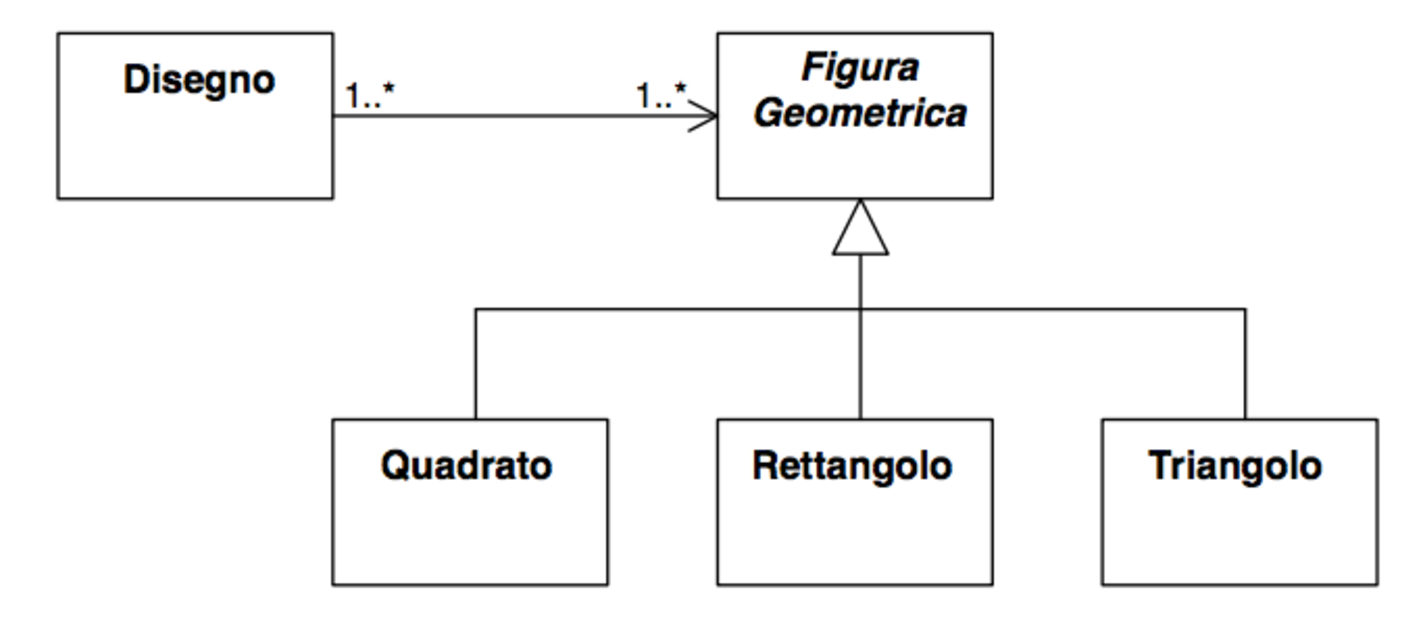
\includegraphics[width=0.7\textwidth]{Img/Generalizzazione.pdf}
      \caption{Generalizzazione tra FiguraGeometrica, Quadrato, Rettangolo e Triangolo.}
      \label{Fig:Generalizzazione}
\end{figure}



%\section{Analisi e progettazione di un sistema}
%Un progetto viene di solito realizzato mediante due fasi distinte:
%\begin{itemize}
%\item \emph{analisi}: vengono identificati gli elementi chiave del \textbf{dominio} del problema
%\item \emph{progettazione}: viene modificato il modello realizato durante la fase di analisi affinche' diventi \textbf{implementabile}
%\end{itemize}
%
%In genere vengono utilizzati le medesime tecniche (UML) ma con livello di dettaglio differente. In confine tra analisi e implementazione non e' netto.
%
%\subsection{La fase di analisi}
%Esistono diverse tecniche per eseguire l'analisi del problema.
%
%
%\begin{itemize}
%\item approcci \textbf{grammaticali} consistono in una analisi della descrizione del linguaggio naturale
%\item approcci basati sull'identificazione degli \textbf{elementi tangibili} (classi potenziali) del dominio applicativo
%\item approcci basati sull'identificazione dei \textbf{comportamenti} dei vari oggetti
%\item approcci basati sull'identificazione degli \textbf{scenari} del sistema
%\item approcci basati sull'identificazione degli \textbf{elementi} e delle loro \textbf{relazioni}
%\end{itemize}







\section{Esercizi}

\subsection{Esercizio: Veicolo-Motore}

\Esercizio{
Progettare il class diagram nella seguente situazione:
\begin{itemize}
\item Un Veicolo \`e composto da un Motore
\item Veicolo: ha una targa e un numero di telaio Motore: ha una cilindrata definita su n pistoni
\item Un Pullman \`e un tipo di Veicolo che trasporta passeggeri 
\item Pullman: appartiene ad una societ\`a e dispone di n posti a sedere 
\item Passeggero: \`e identificato da un nome e cognome
\end{itemize}}


\begin{figure}[h!]
  \centering
    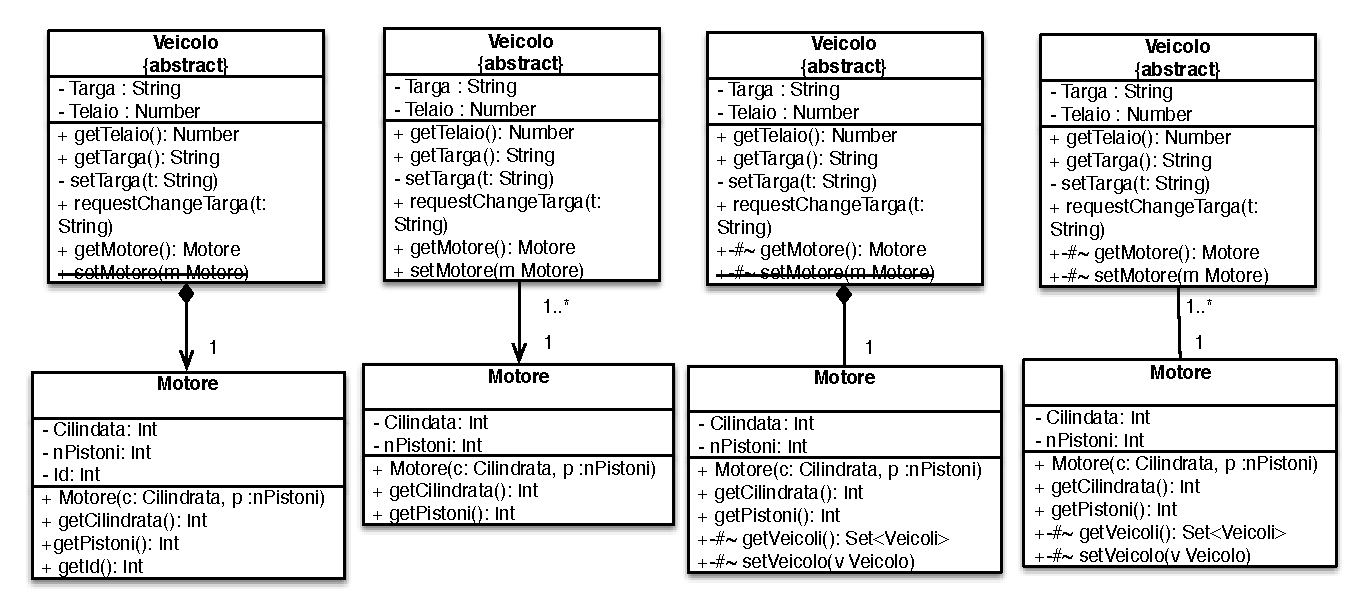
\includegraphics[width=1\textwidth]{Img/motoreveicolo.pdf}
      \caption{Un semplice esempio di gerarchia.}
      \label{Fig:motoreveicolo}
\end{figure}
Identifichiamo le entit\`a in gioco: le potenziali \texttt{classi}. Nel caso in questione identifichiamo tre potenziali classi: \texttt{Veicolo}, \texttt{Pullman} e \texttt{Motore}. Iniziamo analizzando la classe \texttt{Motore}.
Iniziamo discutendo la parte relativa a \texttt{Motore} e  \texttt{Veicolo}. Alcune soluzoni sono presentate in Figura~\ref{Fig:motoreveicolo}.

Il \texttt{Motore} ha una cilindrata definita su n pistoni. La cilindrata \`e normalmente espressa in $cm^3$ mediante un valore maggiore di $0$, per questo scegliamo di memorizzarla per mezzo di un numero intero. Effettuiamo la stessa scelta relativamente al numero di pistoni. Cilindrata e pistoni sono accessibili mediante i metodi \texttt{getCilindrata()} e \texttt{getPistoni()}. Potrebbe sorgerci il dubbio che sia necessario memorizzare un identificativo del motore \texttt{id}, mediante per esempio un intero. Ovviamente la scelta dipende dal ``problema" specifico considerato. Supponiamo di considerare un auto-officina, in tal caso il numero identificativo del motore consente di tener traccia dei motori aggiunti-rimossi dalle varie automobili, della lista di motori in magazzino etc. Se consideriamo invece un sito web, che consente di confrontare i vari tipi di autovetture, l'identificazione del numero seriale del motore non \`e utile per i fini prescelti.

Il \texttt{Veicolo} ha una targa e un telaio. Scegliamo di memorizzare la \texttt{Targa} per mezzo di un attributo di tipo \texttt{String} e il \texttt{Telaio} per mezzo di un attributo di tipo \texttt{Number}. Modellizziamo il \texttt{Veicolo} per mezzo di una classe \texttt{abstract}. Questo perch\`e ci immaginiamo ci siano delle sottoclassi, per esempio \texttt{Pullman} che estenderanno la classe astratta \texttt{Veicolo} rappresentando particolari categorie di veicoli. I metodi \texttt{getTelaio()} e \texttt{getTarga()} permettono di ottenere telaio e tarda del veicolo. Il metodo \texttt{getMotore} consente di ottenere il corrispondente motore. Possiamo fornire il metodo \texttt{setTarga()} se richesto o \texttt{requestChangeTarga()} se per esempio nella specifica \`e richiesto di modellizzare un procedimento nel quale per cambiare una targa bisogna contattare una motorizzazione etc\footnote{In tal caso sarebbe necessario modellizzare anche tali elementi}. L'utilizzo del metodo \texttt{setMotore}  \`e rischioso nel caso in cui si utilizzi una composizione. Infatti nel caso della composizione bisogna garantire che nel momento della distruzione di un veicolo anche il corrispondente motore viene distrutto con esso. Bisogna stare molto attenti a chiamare il metodo setMotore visto che si corre il rischio che il reference di motore sia visibile a classi esterne. Per questo se si desidera esporre tale metodo  \`e necessario farlo con prudenza (metterlo protected), richiamarlo solo da opportune factories etc. Inoltre, per lo stesso motivo, \`e bene che il metodo \texttt{getMotore} ritorni una copia del motore del veicolo.

Riguardo alla relazione tra la classe \texttt{Veicolo} e motore abbiamo tre possibili scelte: associazione ``semplice", aggregazione e composizione. Con l'associazione specifichiamo che a un automobile \`e associato uno specifico motore. L'associazione \`e la relazione ``pi\`u leggera" tra le tre. L'aggregazione indica che un Veicolo aggrega un motore. Per esempio potremmo dire che un veicolo aggrega un telaio,  delle ruote e un motore. Infine la relazione pi\`u forte \`e la composizione. La composizione specifica che quando distruggiamo il veicolo distruggiamo anche il corrispettivo motore. Riguardo alle molteplicit\`a \`e evidente che un veicolo ha uno e un solo motore. Nel caso in cui il motore rappresenti una specifica istanza di un particolare motore (identificato da un serial number), il motore appartiene a uno e un solo veicolo. In quel caso la composizione risulta la scelta pi\`u ragionevole: quando distruggiamo un auto distruggiamo anche il corrispondente motore. Tuttavia, nel caso in cui un motore rappresenti una istanza di un particolare tipo di motore (ma non un motore specifico) \`e possibile dire che da 1 a n macchine montano quel tipo di motore. In quel caso \`e richiesto l'uso dell'associazione.  \`E infine possibile specificare la direzione di navigabilit\`a dell'associazione. Nei primi due casi \texttt{Veicolo} ha il reference al corrispondente \texttt{Motore} ma il motore non conosce il/i veicolo/i su cui \`e montato. Negli ultimi due casi la relazione \`e navigabile in entrambe le direzioni. La traduzione in Java viene lasciata al lettore, seguendo le indicazioni date nell'introduzione.

Discutendo la classi  \texttt{Pullman} e  \texttt{Passeggero}. Alcune soluzoni sono presentate in Figura~\ref{Fig:pullmanPasseggero}.

Il \texttt{Pullman} \`e uno specifico tipo di \texttt{Veicolo}, quindi \texttt{Pullman} estende  \texttt{Veicolo}. \texttt{Pullman} eredita tutti i metodi e gli attributi di \texttt{Veicolo}. A tutti gli effetti un \texttt{Pullman}  \`e un  \texttt{Veicolo}. Un \texttt{Pullman} ha delle caratteristiche  aggiuntive: ha un numero di posti (intero), una societ\`a (stringa) etc. I metodi \texttt{getSociet\`a} e \texttt{setSociet\`a} permettono di settare e ottenere la societ\`a relativa a un pullman. Un \texttt{Passeggero} \`e identificato da un nome e un cognome. 

Discutiamo ora la relazione tra \texttt{Pullman} e \texttt{Passeggero}. La specifica \`e ambigua e si presta a varie interpretazioni che risultano in class diagram differenti. In Figura~\ref{Fig:pullmanPasseggero} ne vengono presentati alcuni. La prima interpretazione \`e che il nostro sistema debba tenere traccia dei passeggeri presenti in un pullman in uno specifico istante temporale. In questo caso, la prima e la seconda soluzione risultano adeguate: esiste una associazione tra le classi \texttt{Pullman} e \texttt{Passeggero}, un passeggero \`e su un pullman e un pullman pu\`o contenere un certo numero di passeggeri. La differenza tra le due soluzioni concerne la navigabilit\`a dell'associazione. Nel primo caso la classe Pullman contiene un reference a ogni passeggero contenuto nel pullman, ma il passeggero non contiene il reference al pullman in cui si trova. Questa soluzione \`e preferibile quando l'associazione deve \emph{solo} essere percorsa in questa direzione, infatti dato un passeggero, per sapere su quale pullman si trova devo scorrere tutti i pullman e controllare che il passeggero non sia all'interno. Nel secondo caso il passeggero contiene il reference al pullman in cui si trova, quindi dato un passeggero \`e semplicissimo sapere il pullman dove si trova. Lo svantaggio \`e in fase di aggiornamento dei passeggeri contenuti in un pullman: bisogna garantire che i reference contenuti nella classe pullman e il reference nella classe passeggero siano consistenti. Per esempio per muovere un passeggero \texttt{p} da un \texttt{pullman1} a un \texttt{pullman2} bisogna eseguire il seguente aggiornamento.

\begin{lstlisting}
pullman1.delPasseggero(p);
pullman2.addPasseggero(p);
p.changePullman(pullman2);
\end{lstlisting}

Nota che senza la terza istruzione si raggiungerebbe una situazione di inconsistenza. La traduzione in Java viene lasciata al lettore, seguendo le indicazioni date nell'introduzione.

\begin{figure}[h!]
  \centering
    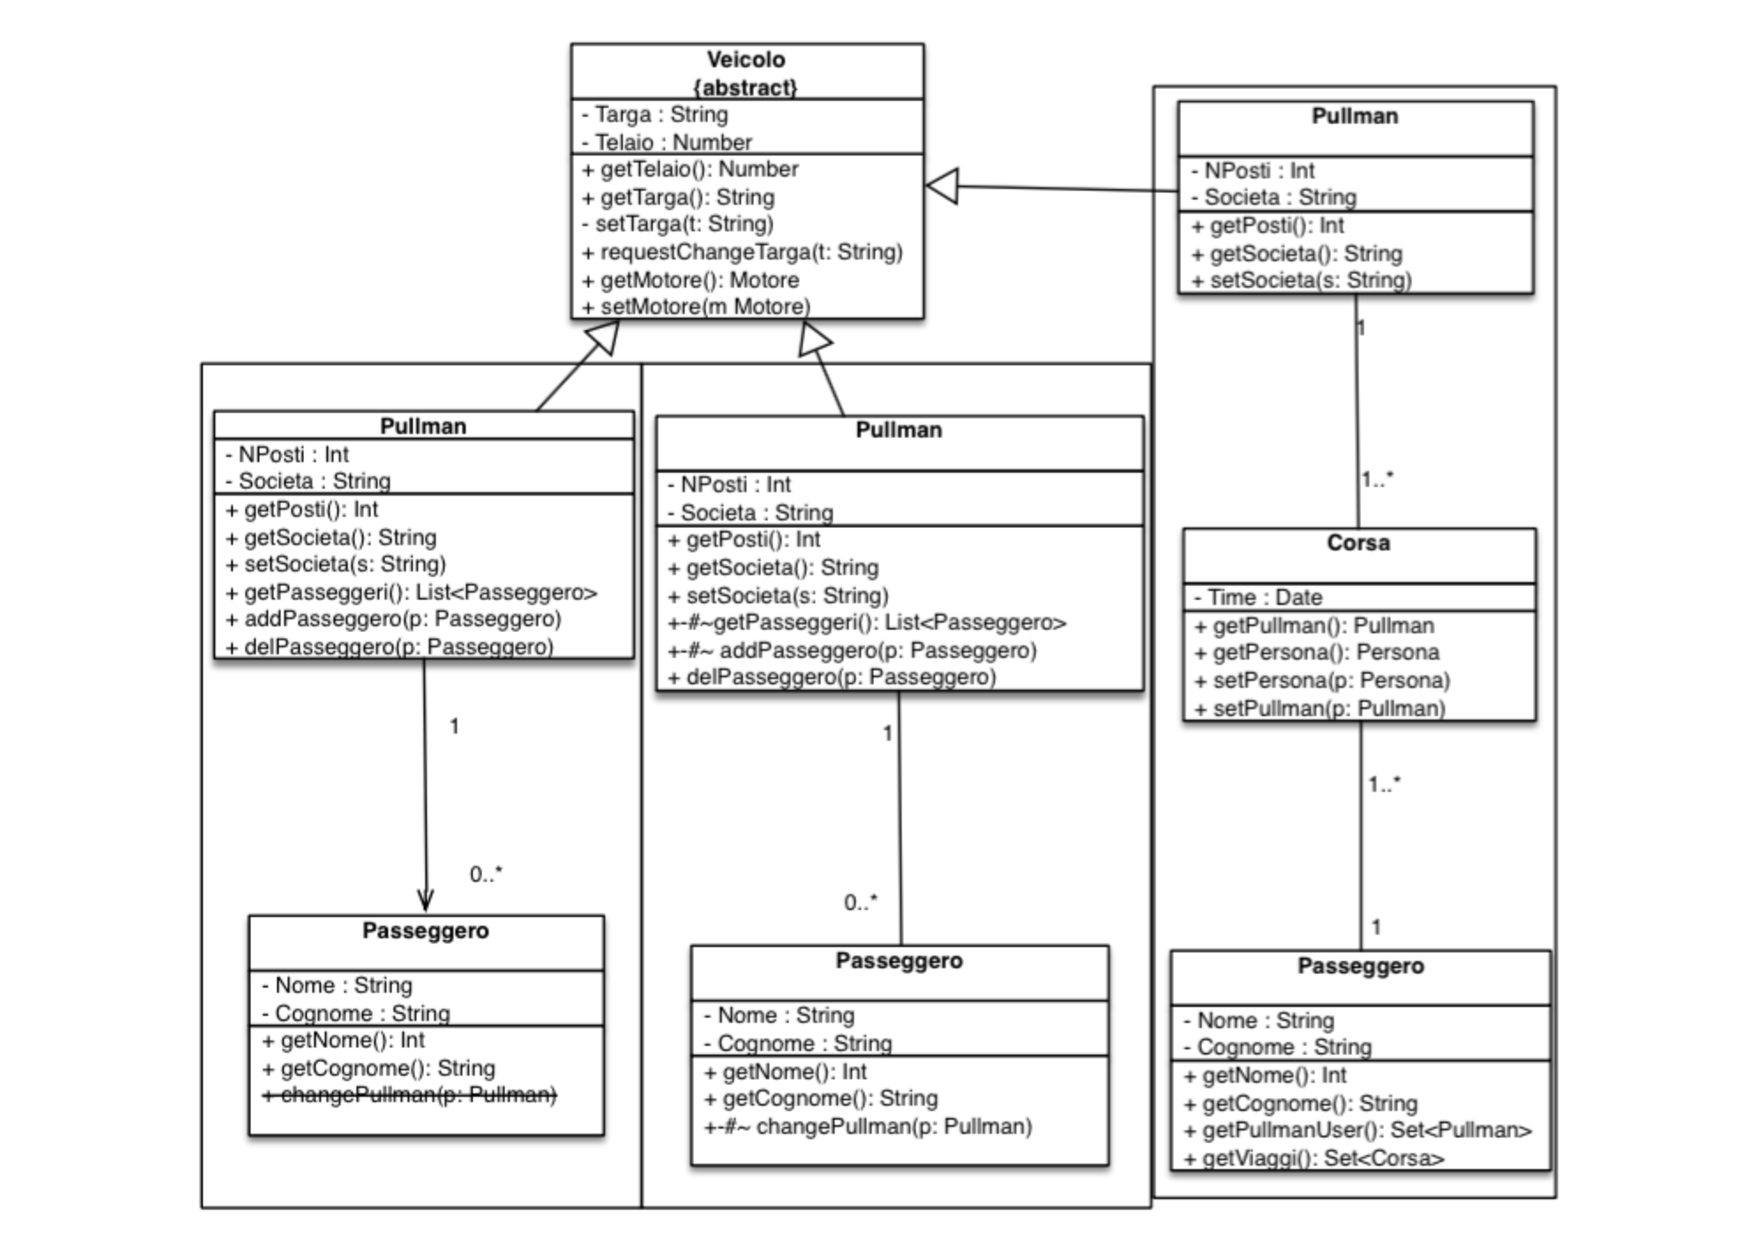
\includegraphics[width=1\textwidth]{Img/pullmanpasseggero.pdf}
      \caption{Pullman passeggero.}
      \label{Fig:pullmanPasseggero}
\end{figure}

\clearpage
\subsection{Esercizio: Giornalisti}
\Esercizio{
\begin{itemize}
\item \emph{R1}: Nella redazione di una testata giornalistica ci sono tre tipi di giornalisti: gli editori, i reporter, ed i fotografi.
\item \emph{R2}: Ogni dipendente \`e caratterizzato da un nome e da un salario e ha diritto ad almeno un benefit (cio\`e un oggetto che viene concesso in uso al dipendente dall'azienda, ma che \`e di propriet\`a dell'azienda).
\item \emph{R3}: Ci possono essere vari tipi di benefit: telefono cellulare, macchina fotografica, computer (che pu\`o essere o un portatile, o un palmare).
\item \emph{R4}: Tra i benefit ci possono anche essere degli apparecchi che hanno funzionalit\`a sia di telefono cellulare che di macchina fotografica.
\item \emph{R5}: Un telefono cellulare \`e caratterizzato da un numero di telefono, e offre la funzionalit\`a di chiamata di un altro numero, e di spedizione di un testo ad un altro telefono.
\item \emph{R6}: Se il telefono ha anche funzionalit\`a di macchina fotografica, permette anche di inviare immagini (sequenze di bit).
\item \emph{R7}: I fotografi hanno diritto, come benefit, ad esattamente una macchina fotografica.
\item \emph{R8}: Ci sono 2 tipi di reporter: i reporter junior e quelli senior.
\item \emph{R9}: I reporter junior hanno diritto ad esattamente un telefono cellulare; i reporter senior hanno invece diritto, ad un apparecchio con doppia funzionalita\`a celullare/macchina fotografica.
\item \emph{R10}: Un reporter pu\`o lavorare in coppia con un fotografo, e fa riferimento ad un editore.
\end{itemize}}

Questo esercizio ha lo scopo di proporre diverse soluzioni che soddisfano i requisiti specificati (in generale nella soluzione viene prestata poca attenzione ad attributi e metodi delle specifiche classi, mentre vengono considerate le loro relazioni). In generale possono esserci soluzioni equivalenti allo stesso problema. Le soluzioni in genere differiscono per la loro estendibilit\`a. Infatti lo sviluppatore, di solito, si trova di fronte a una scelta: soddisfare nello specifico ogni minimo requisito (vincoli di relazione tra classi) rendendo l'implementazione molto relazionata al problema che si desidera risolvere o rilassare dei requisiti (vincoli di relazione tra classi) per rendere l'applicazione pi\`u astratta possibile e pi\`u facilmente estendibile. Il buon progettista \`e in grado di effettuare la scelta migliore in relazione al problema che si sta risolvendo. In genere possono essere 
valutate situazioni intermedie che vincolano il progetto ma rendono comunque l'applicazione estendibile (in certe direzioni).

Consideriamo i requisiti riguardanti i \texttt{Benefit}: \emph{R3}, \emph{R4}, \emph{R5} e \emph{R6}. La soluzione naive, che rispetta perfettamente le specifiche \`e presentata in Figura~\ref{Fig:benefit1}.  Il requisito \emph{R6} specifica che se il telefono ha la funzione di macchina fotografica fornisce una funzionalit\`a che consente di mandare immagini. Il sospetto che ci sorge \`e che anche il computer possegga questa funzionalit\`a di mandare immagini.

\begin{figure}[h!]
  \centering
    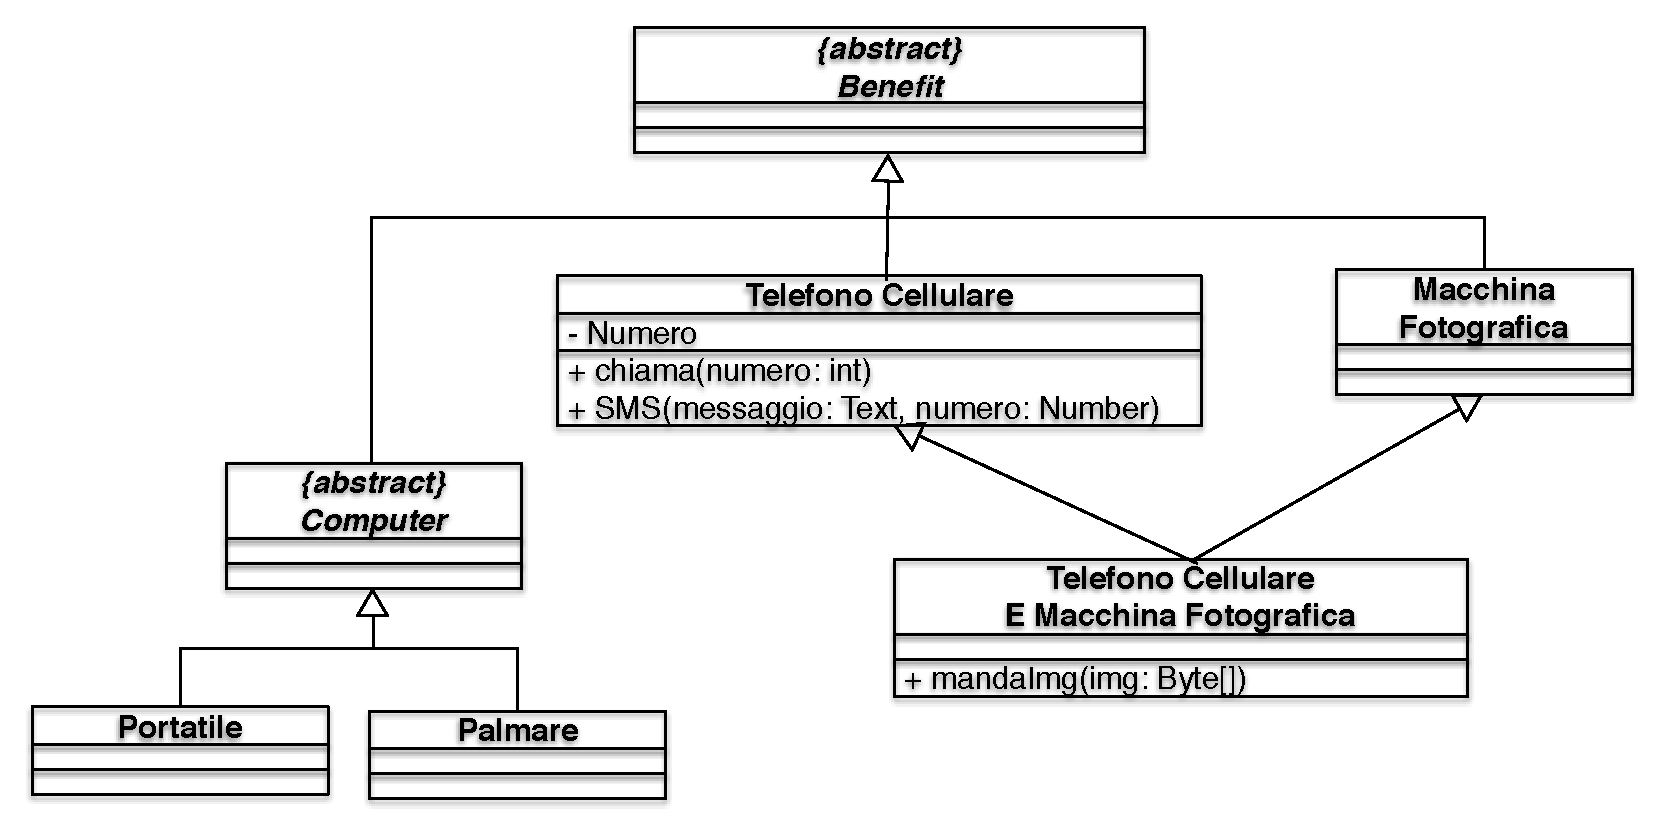
\includegraphics[width=1\textwidth]{Img/benefit1.pdf}
    \caption{Benefit soluzione 1.}
      \label{Fig:benefit1}
\end{figure}
Partendo da questa ipotesi un progettista potrebbe astrare e realizzare il design presentato in~Figura~\ref{Fig:benefit2}. In particolare, lo sviluppatore potrebbe specificare che un \texttt{Benefit} ha delle funzionalit\`a. In questo caso un aggregazione o una composizione \`e il tipo di associazione pi\`u adatta. Le funzionalit\`a e i benefit sono specificate in due gerarchie distinte. Ovviamente in questo caso siamo molto pi\`u flessibili, potremmo aggiungere la funzionalit\`a chiamata a un particolare computer munito di scheda SIM, ma abbiamo meno garanzie ``statiche": potenzialmente una macchina fotografica potrebbe chiamare. In particolare in questo caso \`e molto importante \emph{come} gli oggetti vengono creati e quindi il creational pattern usato.
\begin{figure}[h!]
  \centering
    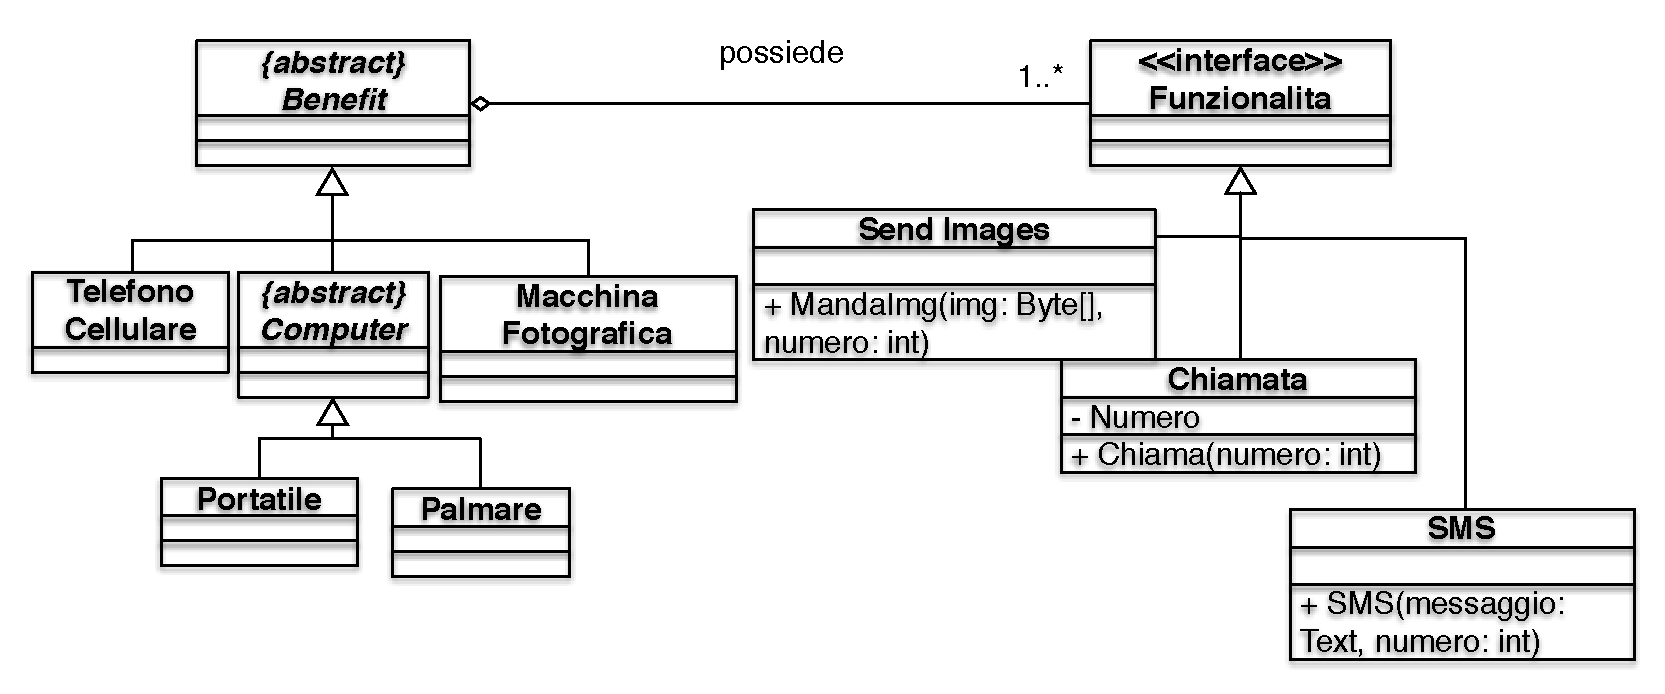
\includegraphics[width=1\textwidth]{Img/benefit2.pdf}
    \caption{Benefit soluzione 2.}
      \label{Fig:benefit2}
\end{figure}
\clearpage
Consideriamo ora i requisiti relativi ai dipendenti: \emph{R1}, \emph{R8}, \emph{R10}.  La prima soluzione che ci viene in mente \`e indicata in Figura~\ref{Fig:dipendente}. Abbiamo una gerarchia di dipendenti e una associazione tra editore e reporter e fotografo e reporter. In questo caso associazione e composizione non sono adeguate. 
\begin{figure}[h!]
  \centering
    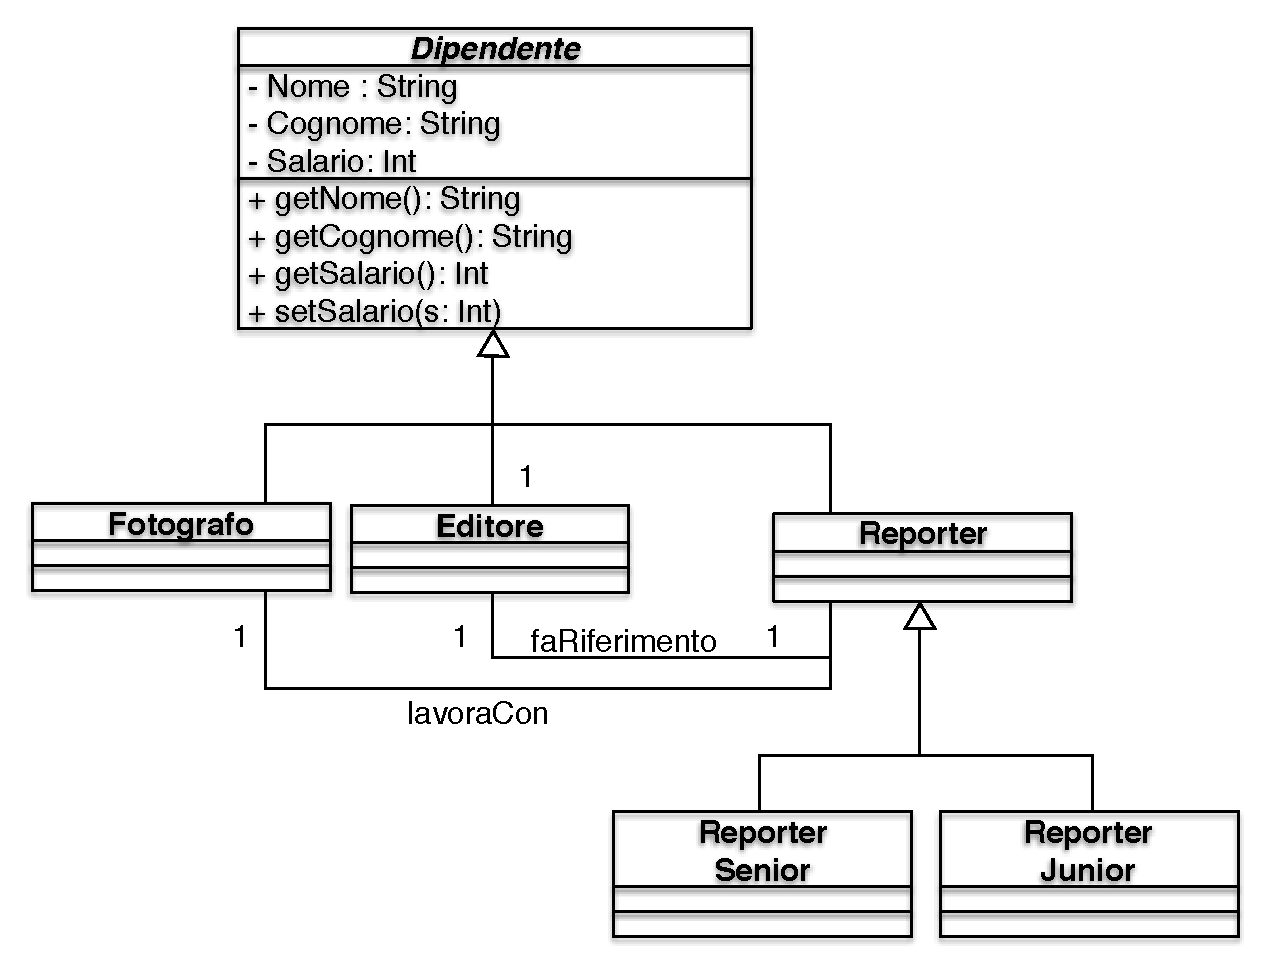
\includegraphics[width=0.7\textwidth]{Img/dipendente.pdf}
 \caption{Dipendente.}
      \label{Fig:dipendente}
\end{figure}

Potremmo tuttavia cercare di astrarre  spostando le relazioni \emph{faRiferimento} e \emph{lavoraCon} verso l'alto (sulla classe dipendente) per rendere le associazioni pi\`u generiche. Una possibile soluzione \`e presentata in Figura~\ref{Fig:dipendente2}. La prima osservazione riguardo a questa soluzione riguarda  l'enumerazione. L'enumerazione non \`e la scelta pi\`u adatta per il caso in questione, e il suo uso va ``limitato". In generale il polimorfismo \`e uno strumento molto potente e ci garantisce grande estendibilit\`a. Nel caso specifico non possiamo per esempio aggiungere il metodo \texttt{getNumeroFotografie()} che \`e un metodo specifico di un fotografo ma non di un editore o un reporter. Questa limitazione pu\`o essere raggirata reinserendo la gerarchia tra i diversi dipendenti e lasciando le relazioni sulla classe dipendente. Tuttavia bench\`e lo spostamento delle relazioni abbia reso il nostro design pi\`u flessibile pu\`o portarci a situazioni inconsistenti, dove un fotografo fa riferimento ad un altro fotografo o un fotografo lavora direttamente con un editore. In questo caso la soluzione descritta in Figura~\ref{Fig:dipendente} \`e preferibile.
\begin{figure}[h!]
  \centering
    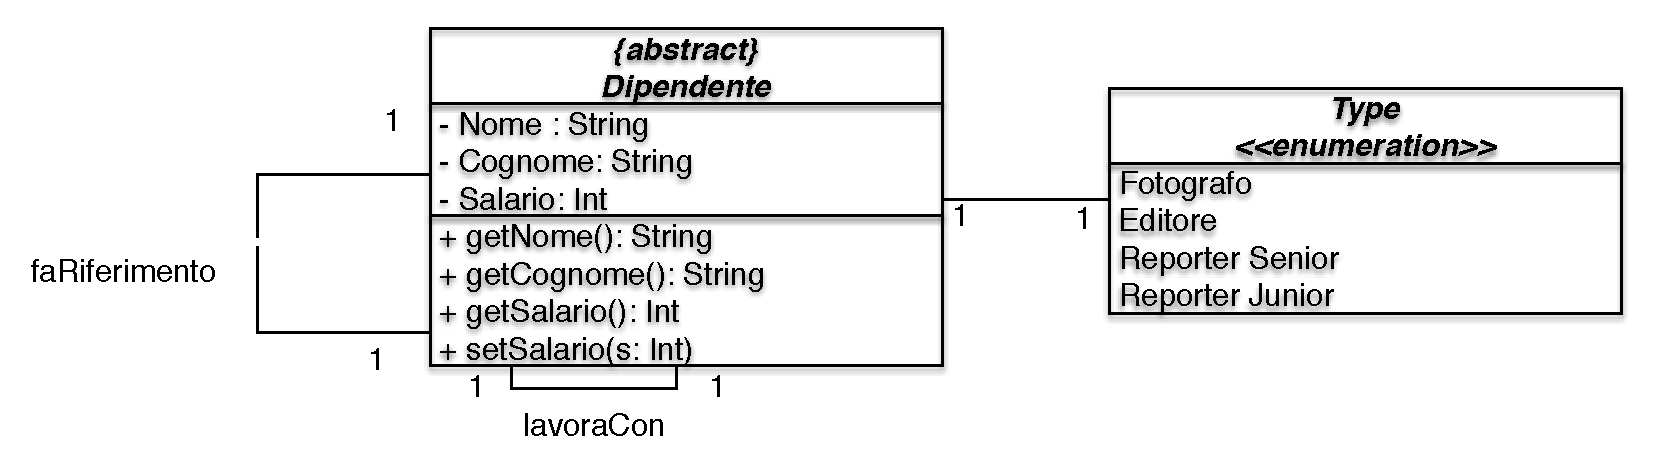
\includegraphics[width=0.7\textwidth]{Img/dipendente2.pdf}
 \caption{Dipendente.}
      \label{Fig:dipendente2}
\end{figure}
\clearpage
Infine analizziamo la relazione tra impiegato e benefit: requisiti \texttt{R2}, \texttt{R7}, \texttt{R9}. La prima soluzione che soddisfa le richieste \`e presentata in Figura~\ref{Fig:dipendentebenefit}. Tuttavia, sembra pi\`u che naturale considerare rilassamenti di questi requisiti: anche a un reporter mandato in guerra verr\`a assegnata una macchina fotografica. Per questo \`e possibile porre un unica associazione tra giornalista e benefit, e forzare le specifiche relazioni per esempio mediante un opportuno creational pattern (la specifica del class diagram corrispondente viene lasciata al lettore).
\begin{figure}[h!]
  \centering
    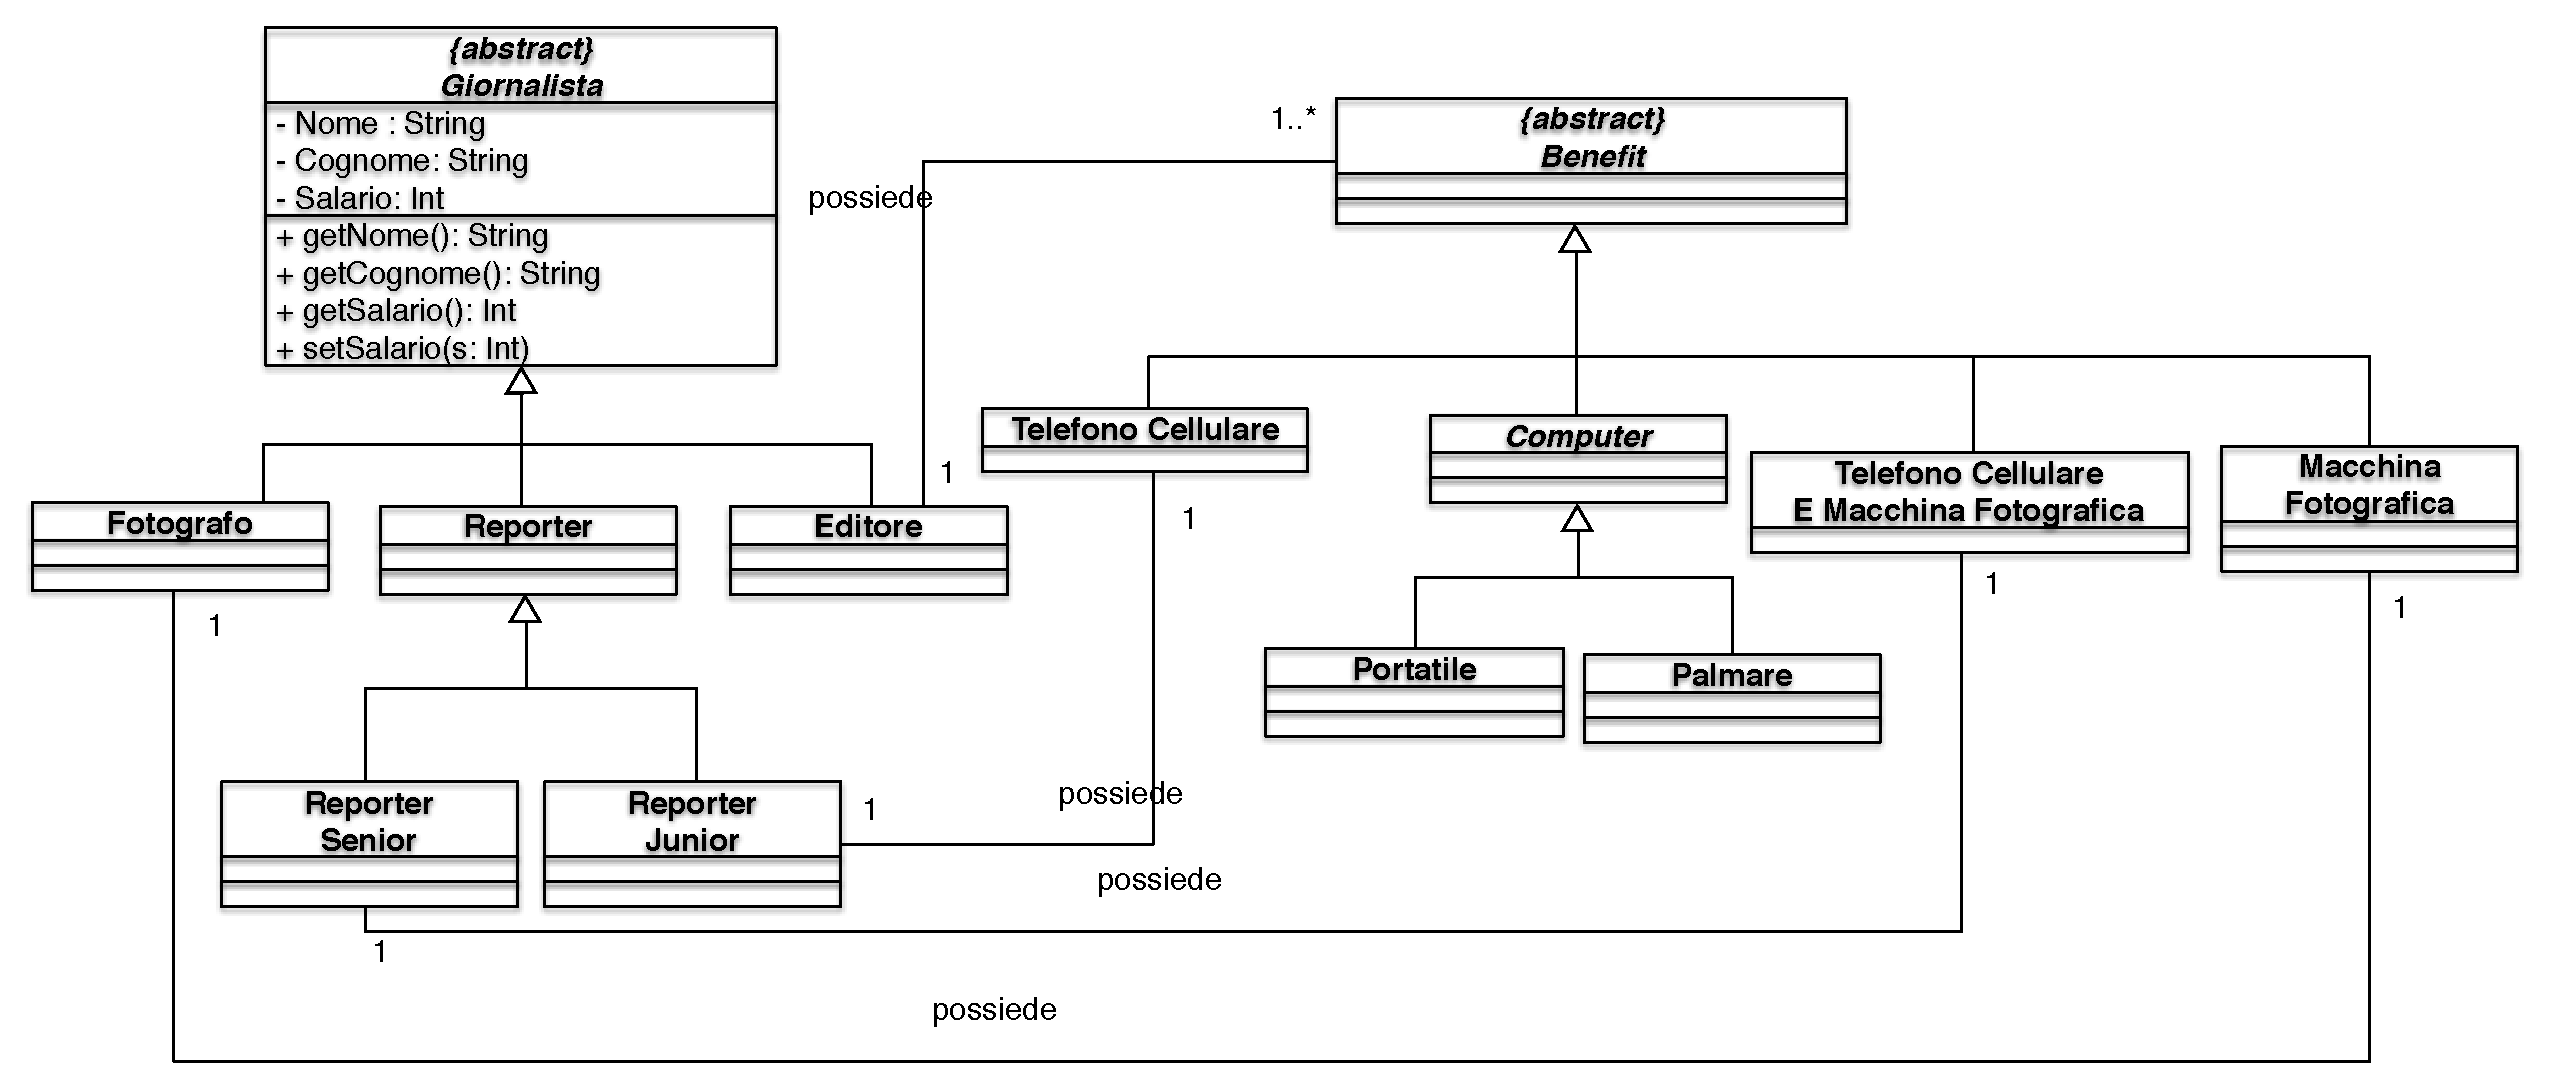
\includegraphics[width=1\textwidth]{Img/impiegatobenefit.pdf}
 \caption{Dipendente.}
      \label{Fig:dipendentebenefit}
\end{figure}
\clearpage


\subsection{Esercizio: Rete informatica}
\Esercizio{
Disegnare un diagramma delle classi UML che rappresenti una rete di computer.
\begin{itemize}
\item Questa si compone di nodi, i quali possono essere di due tipi: host e router.
\item Gli host sono connessi ad esattemente un router, mentre i router possono essere connessi ad un numero qualunque di host e ad almeno un altro router.
\item I nodi di una rete possono essere collegati tra loro mediante link fisici.
\item Un link fisico pu\`o collegare pi\`u host e pi\`u router tra loro.
\item Ogni connessione tra nodi della rete e link fisici è caratterizzata
da un indirizzo IP.
\item Un host nella rete pu\`o offrire dei servizi.
\item Ogni servizio, su un certo host, \`e caratterizzato da una porta.
\item Inoltre, ogni servizio si caratterizza per il tipo di protocollo su cui \`e trasportato, che pu\`o essere TCP o UDP.
\end{itemize}
} 

La soluzione \`e presentata in Figura~\ref{Fig:dipendentebenefit}. Il commento e l'analisi della soluzione \`e lasciata al lettore.
\begin{figure}[h!]
  \centering
    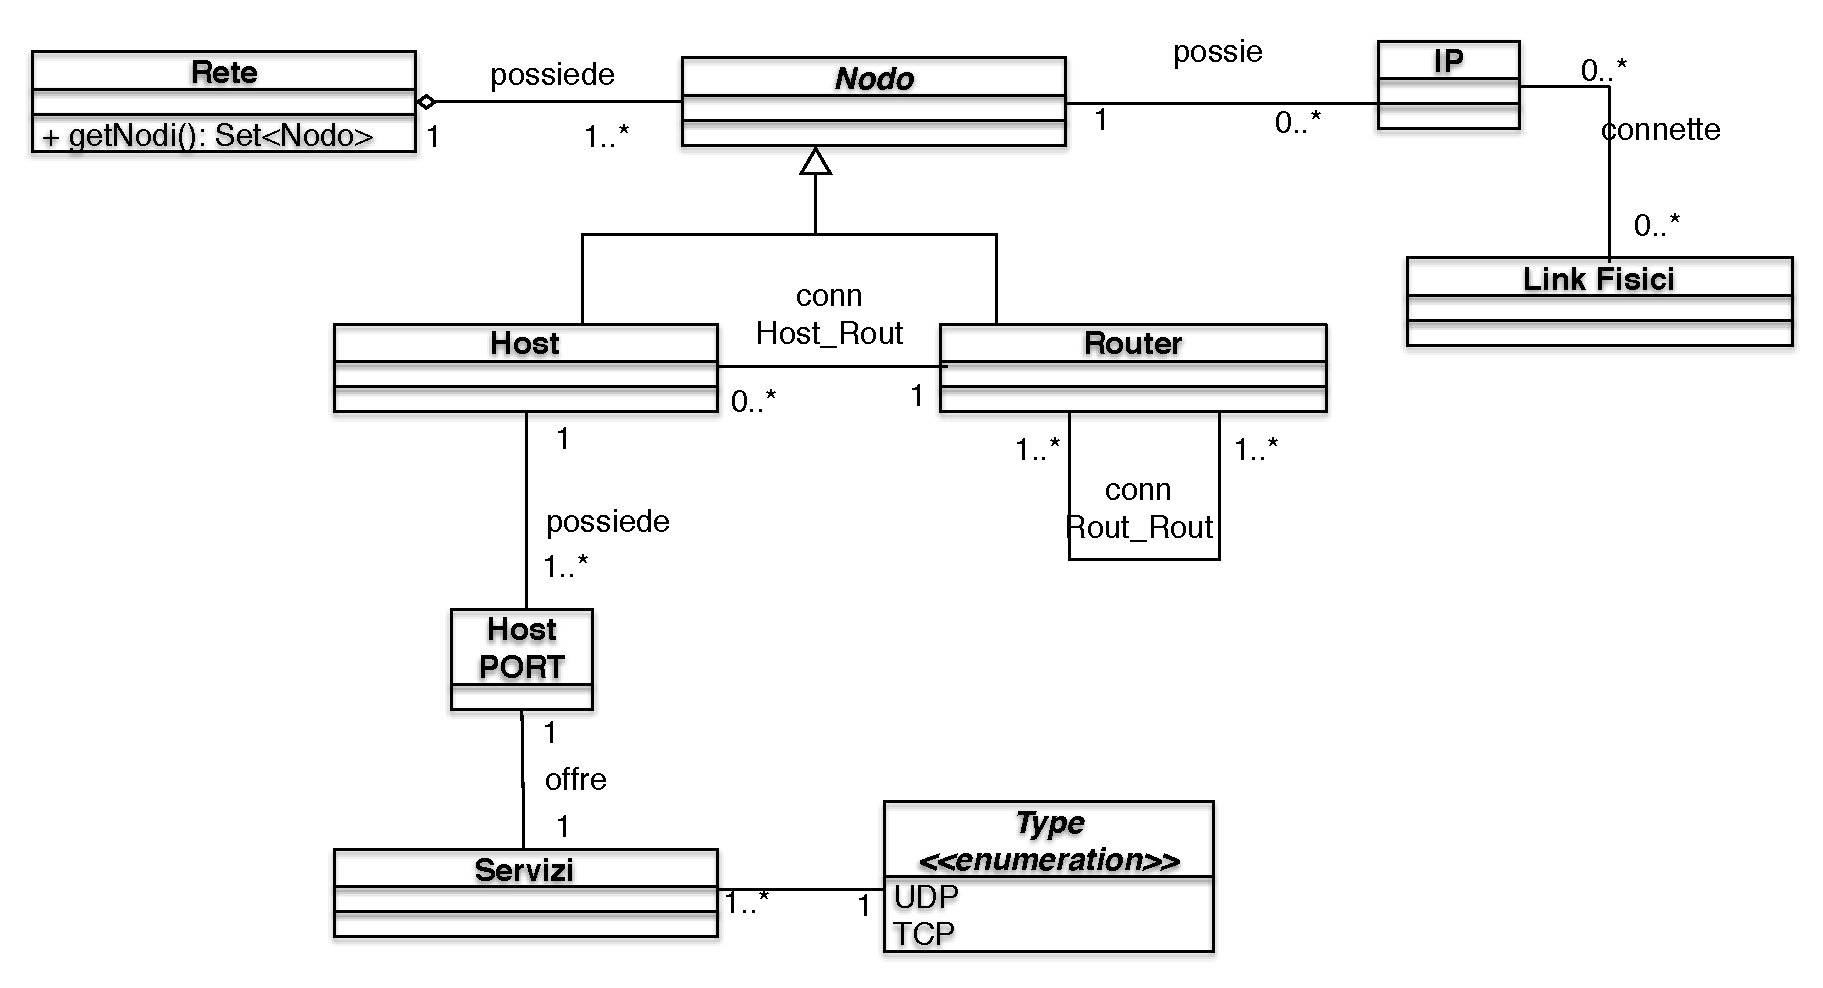
\includegraphics[width=0.8\textwidth]{Img/inf.pdf}
 \caption{Dipendente.}
      \label{Fig:dipendentebenefit}
\end{figure}


\section{Esercizi per casa}
\begin{itemize}
\item implementare le soluzioni proposte.
\item nel caso in cui venga consigliato di utilizzare un creational pattern pensare ed implementare la soluzione utilizzando il pattern considerato adeguato.
\end{itemize}


\clearpage

% ---- Bibliography ----




\addcontentsline{toc}{chapter}{Bibliography}
\bibliographystyle{alpha}
\bibliography{bib}
\nocite{*}


\end{document}

